\documentclass[11pt,a4paper]{article}

% =========================================================
% E-C PlasticKG research manuscript
% Compile with: pdflatex paper.tex (run twice for references)
% Replace every [TO BE FILLED] item with verified project data.
% Do not report placeholder values as experimental findings.
% =========================================================

\usepackage[margin=1in]{geometry}
\usepackage[T1]{fontenc}
\usepackage{lmodern}
\usepackage{microtype}
\usepackage{setspace}
\usepackage{graphicx}
\usepackage{booktabs}
\usepackage{tabularx}
\usepackage{array}
\usepackage{amsmath,amssymb}
\usepackage{enumitem}
\usepackage{float}
\usepackage{caption}
\usepackage{subcaption}
\usepackage{url}
\usepackage{hyperref}
\usepackage[numbers,sort&compress]{natbib}
\usepackage{xcolor}

\hypersetup{
  colorlinks=true,
  linkcolor=blue,
  citecolor=blue,
  urlcolor=blue,
  pdftitle={E-C PlasticKG: An Evidence-Centric and Scope-Aware Knowledge Graph Framework for Plastic Waste Management}
}

\setstretch{1.15}
\setlength{\parskip}{0.35em}
\setlength{\parindent}{1.2em}
\captionsetup{font=small,labelfont=bf}
\renewcommand{\arraystretch}{1.15}

\title{\textbf{E-C PlasticKG: An Evidence-Centric and Scope-Aware Knowledge Graph Framework for Plastic Waste Management}}
\author{
  Anagha C., Gayathri P. S. and Pavithra K.\ M.\\
  \small SODS, Digital University Kerala
}
\date{}

\begin{document}
\maketitle

\begin{abstract}
Studies of plastic-waste management report findings across many abstracts, and those findings often depend on the polymer and the conditions used. Comparing them is not straightforward: a result can look different when its experimental context or supporting passage is overlooked. We present E-C PlasticKG, a prototype that builds topic-specific knowledge graphs from plastic-waste literature. It searches a local OpenAlex collection with TF--IDF ranking and synonym expansion, then uses sentence-level rules to identify candidate claims and entities. The resulting JSON graphs connect claims to source passages, uncertainty labels, selected scope attributes and possible relations to other claims. Through a Flask interface, users can search by keyword, explore the graphs and inspect triples alongside their evidence. We describe the prototype and set out how its extraction, evidence links, scope and uncertainty labels, claim relations and graph structure can be evaluated.
\end{abstract}

\noindent\textbf{Keywords:} Plastic waste management; knowledge graph; evidence grounding; scientific claim extraction; provenance; uncertainty modelling; large language models; scope-aware comparison.

\section{Introduction}

Plastic is used in packaging, construction, healthcare, transportation and many other fields. Managing the waste that follows is difficult: collection and sorting are uneven, reuse has limits, and end-of-life treatment remains challenging. Research therefore spans mechanical and chemical recycling, catalytic conversion, thermal treatment and polymer degradation. The findings from these studies are most useful when read alongside the materials and experimental conditions that produced them.

Much of this knowledge is published in scientific papers, but it is usually embedded in prose rather than collected in a common, machine-readable format. To compare studies, a researcher may have to track the polymer, treatment process, temperature, reaction time, catalyst, pH and reported outcome across many documents. Doing this by hand takes time; automating it brings a different risk, since an extracted statement can lose important context.

Knowledge graphs (KGs) connect entities through typed relationships, making it possible to explore information, search by meaning and bring material from different sources together. Studies of automatic KG construction cover the full process, from gathering data and defining an ontology to extracting, resolving, refining and evaluating knowledge \citep{hogan2021,paulheim2017,kgconstruction2023}. More recent work has explored large language models (LLMs) as another way to turn text into structured knowledge \citep{ibrahim2024,kgconstruction2025}. Together, these approaches offer useful tools for organising scientific information in a specific domain.

Even so, a standard subject--predicate--object triple may leave out what matters when experimental findings are compared. Two abstracts might report different degradation outcomes for the same polymer, yet use different temperatures, catalysts, reaction times or solvents. Without those details, context-dependent results can be mistaken for contradictions. Claims are also hard to check when they are stored without the sentence they came from, and a plausible-sounding relation is not necessarily supported by the source.

E-C PlasticKG explores these issues in plastic-waste research. Instead of storing each extracted statement as an unqualified fact, it represents a claim as an assertion connected to its source, supporting text and reported experimental scope. It also records uncertainty and distinguishes relations that support, challenge or refine another claim. These design choices are intended to make the graph easier to inspect and comparisons across studies more cautious.

The work is guided by the following research questions:

\begin{itemize}[leftmargin=*]
  \item \textbf{RQ1:} How accurately can E-C PlasticKG extract entities, scientific claims and relationships from plastic-waste research abstracts?
  \item \textbf{RQ2:} To what extent does explicit evidence verification improve the traceability and factual reliability of extracted claims?
  \item \textbf{RQ3:} Does representing experimental scope improve the quality of comparisons between scientific findings?
  \item \textbf{RQ4:} How effectively can the framework represent uncertainty in extracted scientific claims?
  \item \textbf{RQ5:} How does E-C PlasticKG compare with the selected project baselines in extraction quality, evidence validity, graph integrity and computational cost?
\end{itemize}

The work contributes an evidence-centred representation of scientific claims, links each claim to its source and supporting text, and records selected experimental conditions and the project's U1--U3 uncertainty labels. It also considers scope when assigning SUPPORTS, CHALLENGES and REFINES relations, and sets out a protocol for comparing the framework with project baselines. These are design contributions; their practical value remains to be established through evaluation.

\section{Literature Review and Related Work}

\subsection{Knowledge graph construction}

Knowledge graphs organise information as entities and typed relationships. Building one typically involves collecting and preparing data, defining a schema or ontology, extracting and resolving information, integrating the graph and checking its quality. Surveys stress that the finished graph depends on each of these stages, not just extraction \citep{hogan2021,kgconstruction2023,kgconstruction2025}. An early mistake in entity or relation recognition can carry through to later processing.

Ontologies and taxonomies offer controlled vocabularies and clear semantic structures, which can make representations more consistent. Their limits are practical as well as conceptual: experts must build and maintain them as terminology changes, and detailed claims or experimental context can be lost unless the schema makes room for them.

\subsection{LLM-based knowledge extraction}

Instruction prompts and structured output have made LLMs useful for a wider range of extraction tasks, including identifying possible entities, claims and relations in unstructured text. Recent surveys describe prompting, fine-tuning and hybrid approaches to LLM-supported KG construction, while pointing to reliability and evaluation as unresolved concerns \citep{ibrahim2024,kgconstruction2025}. In scientific work, a generated statement is still only a candidate: the system needs to separate what the source actually says from what a model may infer.

Generated KG is an existing LLM-based pipeline in the project and serves as one of the reference systems. It offers a point of comparison with a workflow that makes evidence and experimental scope less explicit. Its model, prompts, preprocessing, graph schema and run settings need to be recorded separately; they should not be assumed to match E-C PlasticKG.

\subsection{Evidence, assertions and provenance}

Provenance captures where information came from and, in some cases, how it was produced. It matters whenever a user needs to follow a graph statement back to its source \citep{sikos2020}. Research on assertion, evidence and provenance ontologies also points to the value of structured evidence for reproducibility \citep{chhetri2025}. For a scientific KG, a document identifier alone may not be enough; linking a claim to the sentence or passage that supports it gives readers a more direct way to check it.

E-C PlasticKG follows this approach by connecting claims to both evidence text and document identifiers. A deterministic check tests whether the cited passage appears in the corresponding abstract. This makes the source easier to trace, but it cannot establish on its own that the claim is a sound interpretation of the science.

\subsection{Scientific knowledge graphs and experimental context}

Scientific knowledge graphs often deal with specialised concepts whose meaning depends on the context in which a result was obtained. Recent work discusses challenges such as combining heterogeneous sources, extracting knowledge, aligning ontologies, preserving provenance and evaluating scientific KGs \citep{scikg2026}. In plastic-waste studies, the polymer, temperature, reaction time, catalyst and pH can all influence whether two findings can reasonably be compared.

This study brings these concerns together in a graph for plastic-waste research: claims stay linked to evidence and reported experimental conditions, and those conditions inform the comparison of claims. This framing motivates the design; it does not imply that every existing system lacks these features. A systematic review and direct comparison of implementations would be needed to establish how broad the gap is.

\subsection{Positioning of the present study}

Prior work shows why extraction, refinement and evaluation all matter in KG construction, why LLM outputs need reliability checks, and why scientific claims benefit from provenance and context. E-C PlasticKG applies these ideas to plastic-waste abstracts. The planned comparison uses two project baselines; it keeps reproducible, same-data experiments separate from published results obtained on different datasets, which cannot serve as direct numerical benchmarks.

\section{Research Gap, Aim and Objectives}

\subsection{Research gap}

Plastic-waste findings are scattered across documents and often come from different experimental conditions. If a graph records entities and relations but omits their evidence, scope or uncertainty, it becomes harder to judge where a statement came from and when it applies. Even claims about the same polymer or process may not be comparable if the operating conditions differ.

This work addresses the need for a plastic-waste-focused KG workflow that keeps each scientific claim connected to its supporting text, source document and reported experimental conditions. It also makes uncertainty and claim-to-claim relationships explicit, helping readers distinguish evidence-backed statements from claims that are unverified or arise in a different context.

\subsection{Aim}

This research aims to develop and evaluate a knowledge graph framework that organises findings from plastic-waste abstracts while preserving their evidence and experimental context.

\subsection{Objectives}

\begin{enumerate}[leftmargin=*]
  \item To collect and preprocess a corpus of plastic-waste research abstracts.
  \item To organise domain concepts through a structured taxonomy.
  \item To extract scientific claims, entities, relations and relevant experimental-scope attributes.
  \item To associate extracted claims with source evidence and verify the presence of the evidence in the source text.
  \item To represent uncertainty using the project's U1, U2 and U3 categories, according to a documented annotation and classification protocol.
  \item To canonicalise equivalent entity mentions and reduce duplicate graph entities.
  \item To compare claims using scope-aware SUPPORTS, CHALLENGES and REFINES relations.
  \item To construct, validate and export a provenance-aware knowledge graph.
  \item To evaluate the proposed framework against selected project baselines using a manually annotated reference subset.
\end{enumerate}

\section{Proposed Methodology: E-C PlasticKG}

\subsection{Framework overview}

E-C PlasticKG turns research abstracts and their bibliographic metadata into a graph of documents, entities, claims, evidence, scope attributes and claim relations. Its stages separate candidate extraction from deterministic checks, allowing the system to test generated records against the source before adding them to the graph.

\begin{figure}[htbp]
  \centering
  \includegraphics[width=0.95\linewidth]{architecture.png}
  \caption{Architecture of the E-C PlasticKG application.}
  \label{fig:architecture}
\end{figure}

\subsection{Dataset collection}

The initial corpus contains 100 plastic-waste research abstracts collected through OpenAlex. Each is paired with available bibliographic information, including its source identifier and title. The metadata and abstract text are stored separately, with identifiers linking each processed text to its source record.

The initial experiments use this 100-abstract collection. To make the dataset reproducible, its record should include the retrieval date, OpenAlex search strategy, inclusion and exclusion rules, language restrictions, duplicate handling and retained metadata fields. Because the system reads abstracts rather than full papers, it cannot recover details that do not appear in those abstracts.

\subsection{Preprocessing and data validation}

Before extraction, the text is checked for missing files, mismatches with the metadata, duplicates, excess whitespace and empty or unusually short abstracts. Keeping the original abstract is important: evidence spans must be checked against the source text, not only a normalised copy.

Preprocessing uses Python utilities, including \texttt{pandas}, regular expressions (\texttt{re}) and \texttt{pathlib}. The validation record should give the counts of metadata records, unique identifiers, missing abstracts and duplicates, as well as any abstracts removed by a minimum-length rule. Those counts need to be checked after cleaning; they should not be inferred from the initial collection size.

\subsection{Dynamic taxonomy construction}

A domain vocabulary helps keep the concepts in plastic-waste research organised. The planned categories include polymers, waste-management processes, treatment technologies, catalysts, operating conditions and outcomes. Candidate concepts can be grouped into a hierarchy or a controlled set of types and then used to guide extraction. In the current implementation comparison, however, the system uses a fixed, manually curated vocabulary rather than a learned taxonomy.

The broader project design allows an LLM running through local Ollama to suggest ways of organising candidate concepts, with Pydantic and JSON available for structural checks. Such suggestions would need review for duplicates, ambiguous groupings and unsupported concepts, and each experiment would need a saved taxonomy version. This assisted taxonomy stage is not described as part of the current rule-based extraction run.

\subsection{Scope-conditioned claim extraction}

Claim extraction looks for scientifically meaningful statements in each abstract. Rather than returning only isolated triples, the prototype creates candidate claim records with an identifier, statement, relevant entities, relation information, source document and any experimental-scope attributes found in the text.

The scope fields considered are polymer, temperature, runtime, catalyst and pH. A value is recorded only when the abstract provides textual support; missing information is left unknown rather than inferred. In the current prototype, sentence-level rules and a curated vocabulary produce the candidate records. If an LLM-based extraction stage is added, its model, prompt, decoding settings, retry policy and output schema will need to be documented separately.

\subsection{Evidence extraction and deterministic verification}

Each candidate claim is linked to evidence from its source abstract. The evidence record retains the source identifier and supporting sentence or passage. A deterministic check then tests whether that text can be found in the original abstract, following the project's matching and normalisation rules.

This check answers a narrow question: can the cited passage be located in the source? It does not show that the passage entails the claim, that the claim is scientifically correct or that the underlying study is methodologically sound. Those questions require human review or a separately validated semantic assessment, so textual traceability and claim correctness are treated as different things.

\subsection{Uncertainty modelling}

Abstracts differ in how directly and precisely they state their findings. E-C PlasticKG records uncertainty with three project-defined labels: U1, U2 and U3. The aim is to avoid presenting every extracted statement as equally certain.

These labels need a written protocol defining each category, the evidence required, how to handle ambiguous cases and what to do when information is missing. The same definitions must be used for system outputs and reference annotations; they should be set before results are examined. Agreement with human labels can then be assessed using macro-F1 and, where appropriate, a chance-corrected agreement statistic.

\subsection{Entity canonicalisation}

Authors may refer to the same polymer, process or chemical by different names, abbreviations or spellings. Entity canonicalisation maps such mentions to a consistent representation, reducing duplicate graph nodes and making queries more useful.

The project uses RapidFuzz to find possible matches based on string similarity. A similarity score is a prompt for review, not proof that two mentions refer to the same thing. Thresholds should be chosen on development data and checked against manually reviewed entity pairs. If sentence embeddings are introduced, their model and version should also be recorded. In all cases, the original wording should be retained.

\subsection{Scope-aware claim comparison}

Once claims have been extracted and entities canonicalised, the framework looks for pairs that may describe related findings. It considers shared entities and the available scope fields: polymer, temperature, runtime, catalyst and pH. A difference in claims is not automatically a contradiction, especially when key conditions differ or are missing.

The framework uses three intended relation labels:
\begin{itemize}[leftmargin=*]
  \item \textbf{SUPPORTS:} one claim provides evidence consistent with or supportive of another claim, within the documented comparison context;
  \item \textbf{CHALLENGES:} one claim reports a finding that is in tension with another claim, after relevant scope differences have been considered;
  \item \textbf{REFINES:} one claim adds detail, qualification or a narrower condition to another claim without necessarily rejecting it.
\end{itemize}

These labels describe how claims relate; they do not imply a causal link between physical entities. The comparison rationale and scope fields used should be recorded. When the available scope is too sparse for a defensible decision, the system should leave the relation unassigned or flag it for review.

\subsection{Knowledge graph construction}

The graph keeps source documents, entities, claims and evidence as distinct nodes. This assertion-centred structure avoids presenting a claim as an unqualified edge between two entities. Claim nodes can store the statement, identifier, uncertainty label and scope attributes; evidence nodes retain the supporting passage and its source.

A conceptual representation is:

\begin{itemize}[leftmargin=*]
  \item \textbf{Document nodes} represent the source abstracts and their metadata.
  \item \textbf{Entity nodes} represent canonical domain concepts such as polymers, processes and catalysts.
  \item \textbf{Claim nodes} represent extracted scientific assertions.
  \item \textbf{Evidence nodes} represent the text spans supporting claims.
  \item \textbf{Claim relations} connect claims through SUPPORTS, CHALLENGES or REFINES labels.
\end{itemize}

The implementation uses NetworkX for graph processing. A directed multigraph is useful when several typed or provenance-bearing edges connect the same nodes, but the exact graph class and schema should be confirmed against the release being evaluated. Stable node and edge identifiers, along with provenance attributes, allow graph records to be traced back to the input.

Figure~\ref{fig:example-graph} shows the Flask interface for a Pyrolysis search. The API returned 19 claims from nine abstracts, while the app displayed 12 subject--predicate--object triples involving nine entities. Users can inspect the associated claims and evidence in the application.
\begin{figure}[htbp]
  \centering
  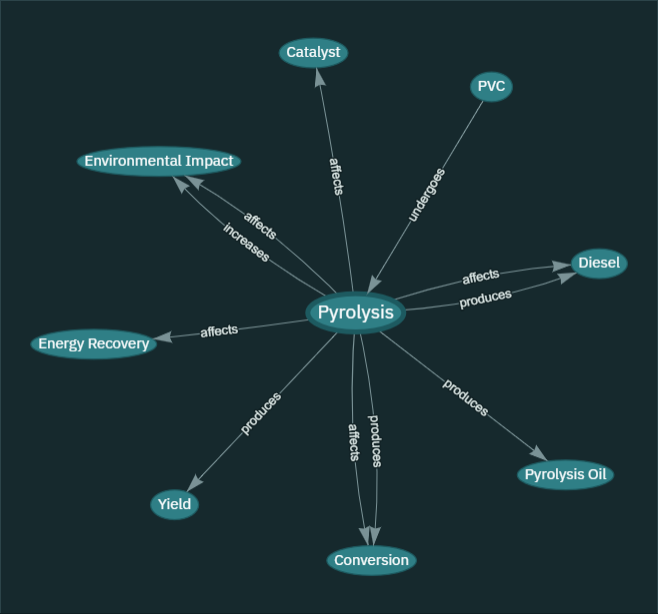
\includegraphics[width=0.78\linewidth]{example-knowledge-graph.png}
  \caption{Pyrolysis knowledge graph rendered by the E-C PlasticKG app.}
  \label{fig:example-graph}
\end{figure}

\subsection{Graph validation and export}

Before export, the graph is checked against its schema: identifiers should be unique, node and edge types permitted, required claim fields present, and document and evidence references valid. Uncertainty and claim-relation labels are also checked against the allowed values. The evidence-check outcome should remain available as a validation attribute or record.

The project plan includes machine-readable export in JSON, GraphML and CSV. Only formats that are generated and validated should be reported. Useful graph summaries include the numbers of documents, entities, claims, evidence records and relations, along with isolated nodes, invalid references and validation failures. These counts describe the graph's structure, not its accuracy; accuracy requires comparison with annotated reference data.

\section{Experimental Setup}

\subsection{Dataset and experimental unit}

The evaluation begins with 100 plastic-waste abstracts from OpenAlex, treating each abstract as the unit for extraction and document-level scoring. A subset of 20--30 abstracts is proposed for manual annotation. The selection procedure (random, topic-stratified or otherwise) needs to be recorded so readers can judge how representative the subset is.

The annotations should cover entities, claims, relations, evidence spans, scope fields and uncertainty labels. At least two annotators should independently label a shared portion of the data, resolve disagreements through adjudication and follow the same written guidelines. They should not see system predictions while preparing the reference labels.

\subsection{Computational environment}

The project is written in Python and the recorded runs use an NVIDIA DGX environment with Python 3.9.16, an NVIDIA A100 80\,GB GPU and CUDA 12.2. The local Ollama configuration identifies Llama 3.1 8B Instruct, with the recorded model tag \texttt{llama3.1:8b-instruct-fp16}. These settings should be confirmed against the logs for the runs ultimately reported.

\begin{table}[htbp]
\centering
\caption{Initial experimental environment. Verify each entry against the final run logs before submission.}
\label{tab:environment}
\begin{tabularx}{\linewidth}{>{\raggedright\arraybackslash}p{0.34\linewidth}X}
\toprule
\textbf{Parameter} & \textbf{Recorded or intended setting}\\
\midrule
Research domain & Plastic waste management\\
Initial corpus & 100 research abstracts\\
Data source & OpenAlex\\
Programming language & Python 3.9.16\\
LLM runtime & Local Ollama\\
LLM & Llama 3.1 8B Instruct (FP16; verify exact tag)\\
GPU environment & NVIDIA DGX; NVIDIA A100 80\,GB\\
CUDA & 12.2 (recorded environment)\\
Graph library & NetworkX\\
Structured validation & Pydantic\\
Entity matching & RapidFuzz\\
\bottomrule
\end{tabularx}
\end{table}

Reproducing the runs also requires package versions, GPU allocation, operating-system and Ollama versions, the model checksum or exact tag, prompt templates and decoding settings, context length, timeout, retry policy and preprocessing configuration. Any differences in models or hardware across the three approaches should be made explicit.

\subsection{Baseline approaches}

The comparison covers two reference approaches alongside E-C PlasticKG:

\begin{enumerate}[leftmargin=*]
  \item \textbf{OntoGen:} an ontology- and taxonomy-generation pipeline. The supplied implementation comparison describes a workflow that processes full-text scientific documents and uses LLM prompts to build vocabularies, category seeds, taxonomies and graph representations.
  \item \textbf{Generated KG:} an existing LLM-based knowledge graph pipeline in the project. Its outputs and run settings still need to be evaluated on the same dataset before quantitative comparisons can be made.
  \item \textbf{E-C PlasticKG:} the plastic-waste-focused prototype, which uses a curated vocabulary and rule-based extraction to build topic-specific claim graphs from OpenAlex abstracts.
\end{enumerate}

The OntoGen--E-C PlasticKG comparison is based on released code and documented behaviour; it is a comparison of design and implementation, not accuracy on a shared benchmark. The descriptive run does not show that either OntoGen or Generated KG was run on the same 100 abstracts with the same annotations and metrics. For that reason, architectural differences are reported separately from output counts, and the systems are not ranked by predictive performance.

\subsection{Fair comparison protocol}

For a fair comparison, each executable approach needs the same input documents, reference annotations, matching rules and metric definitions. Entity and relation matching criteria should be settled before scoring. Where a system is stochastic, repeated runs and their randomisation settings should be reported when feasible.

Output volume alone says little about quality: a larger graph is not necessarily a more accurate one. The main analysis should report precision, recall and F1 against manual annotations, together with evidence validity, scope extraction and graph integrity.

\section{Evaluation Metrics}

\subsection{Entity, claim and relation extraction}

For each task, a true positive (TP) is an extracted item that matches the reference; a false positive (FP) is an unmatched extraction; and a false negative (FN) is a reference item the system missed. Precision, recall and F1 are calculated as follows:

\begin{equation}
\mathrm{Precision}=\frac{TP}{TP+FP}
\end{equation}
\begin{equation}
\mathrm{Recall}=\frac{TP}{TP+FN}
\end{equation}
\begin{equation}
\mathrm{F1}=2\cdot\frac{\mathrm{Precision}\cdot\mathrm{Recall}}
{\mathrm{Precision}+\mathrm{Recall}}
\end{equation}

The evaluation protocol should say whether entities match by canonical identifier, normalised string or adjudicated semantic equivalence. Claim matching should account for meaning and relevant entities, rather than relying only on surface similarity. Relations should be scored against the agreed schema.

\subsection{Evidence verification}

Evidence precision is the proportion of extracted spans accepted by the reference annotations or by the specified source-text check:

\begin{equation}
\mathrm{Evidence\ Precision} =
\frac{\text{Number of valid extracted evidence spans}}
{\text{Total extracted evidence spans}}.
\end{equation}

Evidence coverage is the share of reference claims for which the system supplies an acceptable supporting span:

\begin{equation}
\mathrm{Evidence\ Coverage} =
\frac{\text{Reference claims with valid linked evidence}}
{\text{Total reference claims}}.
\end{equation}

The span-matching rule, whether exact or normalised, should be reported. Finding a passage in the source is not, by itself, evidence of entailment or scientific correctness.

\subsection{Scope extraction}

Scope extraction is assessed for polymer, temperature, runtime, catalyst and pH. Accuracy is suitable when a categorical field has one clear reference value; fields with multiple or partial values call for field-level precision, recall and F1. A value that was not reported should not be counted in the same way as an incorrect prediction.

\subsection{Uncertainty classification}

System U1, U2 and U3 labels are compared with human annotations using per-class precision, recall and F1, as well as macro-F1. The annotation process should also report inter-annotator agreement. Cohen's kappa is one option for two annotators assigning mutually exclusive labels; other designs may require a different statistic.

\subsection{Claim-comparison quality}

Claim relations are scored against manually assigned SUPPORTS, CHALLENGES and REFINES labels. Accuracy and macro-F1 are useful, especially when classes are imbalanced. The annotation guide should explain how to handle cases with too little scope information. A generally plausible relation should not count as correct unless the abstract supports it.

\subsection{Graph integrity and efficiency}

Graph integrity can be measured through schema validity, source references, evidence-link coverage, identifier consistency and the proportion of records passing deterministic checks. Efficiency can be reported as end-to-end runtime and, when available, peak memory use. Hardware and run conditions should either be held constant or described clearly.

\begin{table}[htbp]
\centering
\caption{Evaluation dimensions and proposed metrics.}
\label{tab:metrics}
\begin{tabularx}{\linewidth}{>{\raggedright\arraybackslash}p{0.25\linewidth}XX}
\toprule
\textbf{Evaluation area} & \textbf{Metric} & \textbf{Purpose}\\
\midrule
Entity extraction & Precision, recall, F1 & Correctness and completeness of entity identification\\
Claim extraction & Precision, recall, F1 & Correctness and completeness of scientific claims\\
Relation extraction & Precision, recall, F1 & Correctness of entity and claim relations\\
Evidence & Evidence precision, evidence coverage & Validity and availability of supporting text\\
Scope & Field-level accuracy / precision / recall / F1 & Correctness of experimental conditions\\
Uncertainty & Macro-F1, per-class F1, agreement & Agreement with the uncertainty reference labels\\
Claim comparison & Accuracy, macro-F1 & Correctness of SUPPORTS, CHALLENGES and REFINES labels\\
Graph integrity & Schema validity, provenance coverage & Structural correctness and traceability\\
Efficiency & Runtime, peak memory & Computational cost\\
\bottomrule
\end{tabularx}
\end{table}

\section{Results and Comparative Analysis}

The results below distinguish three kinds of evidence: descriptive counts from the current E-C PlasticKG run, implementation differences from the supplied OntoGen comparison and predictive measures that have not yet been assessed. Graph size and valid source offsets do not replace evaluation against human-reviewed annotations.

\subsection{Dataset and graph statistics}

The dataset contains 100 OpenAlex abstracts. In the descriptive run, the system generated outputs for 22 topic queries. Twenty returned at least one claim; Catalysed Cracking and Sustainable Recycling returned none. Across all topics, there were 121 claim instances. Deduplicating by claim identifier left 95 unique claims linked to 43 abstracts. Pyrolysis had the largest output, with 19 claim instances, followed by Microplastics with 17.

\begin{table}[htbp]
\centering
\caption{Descriptive output statistics from the current E-C PlasticKG run.}
\label{tab:graphstats}
\small
\begin{tabularx}{\linewidth}{>{\raggedright\arraybackslash}Xr}
\toprule
\textbf{Statistic} & \textbf{Observed value}\\
\midrule
OpenAlex abstracts in the initial corpus & 100\\
Configured topic queries & 22\\
Topics producing at least one claim & 20\\
Topics producing no claims & 2\\
Query-level claim instances & 121\\
Unique claim identifiers after deduplication & 95\\
Distinct source abstracts represented by claims & 43\\
Largest topic output: Pyrolysis & 19 claims\\
Largest topic output: Microplastics & 17 claims\\
Evidence edges & 121\\
From-Finding edges & 121\\
Subject edges & 121\\
Has-Object edges & 58\\
Candidate inter-claim relations & 9\\
\bottomrule
\end{tabularx}
\end{table}

The graph contained seven SUPPORTS and two REFINES relations; it produced no CHALLENGES or INCONCLUSIVE relations. Of the 121 claim instances, 101 were labelled U1, 20 U2 and none U3. The run recorded 55 polymer, 2 temperature, 3 reaction-time and 11 catalyst scope occurrences, no medium occurrences, and 9 inherited-from-abstract indicators. These counts can overlap and include claims repeated across topic outputs, so they are neither counts of unique studies nor measures of scope accuracy.

\begin{table}[htbp]
\centering
\caption{Observed uncertainty and scope output distribution.}
\label{tab:scopeuncertainty}
\small
\begin{tabularx}{\linewidth}{>{\raggedright\arraybackslash}Xr}
\toprule
\textbf{Output field} & \textbf{Observed count}\\
\midrule
U1 (low uncertainty) & 101\\
U2 (moderate uncertainty) & 20\\
U3 (high uncertainty) & 0\\
Polymer scope occurrences & 55\\
Temperature scope occurrences & 2\\
Reaction-time scope occurrences & 3\\
Catalyst scope occurrences & 11\\
Medium scope occurrences & 0\\
Inherited-from-abstract indicators & 9\\
\bottomrule
\end{tabularx}
\end{table}

All 121 returned evidence passages matched the corresponding source-text slices at their recorded offsets (121/121; 100\%). This confirms that each passage can be located in its abstract, a useful structural provenance check. It does not measure evidence precision, entailment or claim correctness: a passage can be copied accurately and still be irrelevant to, or misinterpreted as, support for a claim.

\subsection{Implementation-level comparison with OntoGen}

The supplied comparison looks at the released OntoGen workflow alongside E-C PlasticKG. The systems have related but distinct aims: OntoGen derives vocabularies and hierarchical taxonomies from full-text scientific documents, while E-C PlasticKG builds keyword-specific claim graphs from OpenAlex abstracts and links claims to evidence and selected experimental conditions.

\begin{table}[htbp]
\centering
\caption{Implementation-level comparison of OntoGen and E-C PlasticKG based on the supplied released-code comparison.}
\label{tab:implementationcomparison}
\scriptsize
\begin{tabularx}{\linewidth}{>{\raggedright\arraybackslash}p{0.19\linewidth}XX}
\toprule
\textbf{Aspect} & \textbf{OntoGen (reference)} & \textbf{E-C PlasticKG (proposed)}\\
\midrule
Primary purpose & Builds a topic taxonomy and ontology from scientific literature. & Builds keyword-specific, claim-centred graphs that retain evidence and selected experimental conditions.\\
Input & Full-text PDFs converted to text; abstract and introduction sections are used in the documented workflow. & 100 OpenAlex abstract records stored with identifiers, titles and abstract text.\\
Extraction engine & LLM prompting through Ollama; released examples document Llama models including 70B configurations, with optional external API use. & Rule-based extraction using a curated 53-entry domain lexicon, regular expressions, cue words and sentence-level rules; no LLM is used in the described extraction stage.\\
Knowledge unit & Terms, definitions, category assignments and term--relation--term structures. & Sentence-level scientific claim candidates linked to subject/object entities and source evidence.\\
Vocabulary & Open vocabulary induced from the input documents. & Fixed, manually curated plastic-waste vocabulary.\\
Hierarchy and types & LLM-generated category seeds and taxonomy classification, including is-a relationships. & No learned taxonomy in the compared implementation; seven fixed entity types: Polymer, Process, Catalyst, Product, Monomer, Outcome and Concept.\\
Relations & is-a and short free-text relations among extracted terms. & Structural edges (Subject, Has Object, Evidence, From Finding) and claim-level labels (Supports, Challenges, Refines, Inconclusive).\\
Cross-document handling & Merges vocabulary across documents into a shared taxonomy using synonym identifiers. & Produces separate topic graphs and compares claims across abstracts when selected subject/object entities match.\\
Evidence and provenance & Tracks term positions and flags unmatched terms; taxonomy nodes do not retain a claim-specific evidence passage in the compared representation. & Links each claim to a verbatim evidence sentence, abstract identifier/title and character offsets.\\
Experimental scope & Not explicitly modelled in the compared workflow. & Captures polymer, temperature, reaction time, catalyst and medium; values found elsewhere in an abstract can be marked as inherited.\\
Uncertainty & No explicit U1/U2/U3 field in the compared workflow. & Assigns three uncertainty levels (U1, U2 and U3) using lexical hedging cues.\\
Retrieval and interface & Corpus/topic input followed by numbered scripts and notebooks. & Keyword, synonym expansion and TF--IDF retrieval; separate topic graphs served through a Flask web interface and CLI export.\\
Execution profile & LLM inference through Ollama; GPU use is documented for larger model configurations. & CPU-oriented Python/Flask execution in the compared implementation.\\
Evaluation support & Released notebooks include term-extraction and taxonomy-oriented evaluation routines. & Current descriptive run is supplemented by preliminary, unverified metrics on 30 abstracts; no completed shared gold-standard benchmark is available.\\
\bottomrule
\end{tabularx}
\end{table}

The comparison points to different design priorities, not a winner. OntoGen offers a more open-ended, taxonomy-focused workflow with LLM-assisted vocabulary and hierarchy construction. E-C PlasticKG focuses more on claim-level evidence, selected experimental conditions and explicit uncertainty fields. These differences explain the motivation for E-C PlasticKG but say nothing about which system extracts claims more accurately. A quantitative comparison would first need aligned inputs, a mapping between the output schemas and a shared, human-reviewed reference set.

\subsection{Preliminary annotation-based evaluation and metric status}

We also ran the existing rule-based E-C PlasticKG extractor against an evaluation workbook covering 30 abstracts. The workbook is marked ``PRELIMINARY - UNVERIFIED DRAFT'', so the figures below are provisional diagnostics, not final gold-standard scores. It contains no evaluation of OntoGen or Generated KG.

\begin{table}[htbp]
\centering
\caption{Preliminary E-C PlasticKG evaluation on 30 abstracts. Results are unverified and must not be interpreted as final benchmark scores.}
\label{tab:preliminarymetrics}
\small
\begin{tabularx}{\linewidth}{>{\raggedright\arraybackslash}Xr}
\toprule
\textbf{Metric} & \textbf{Preliminary result}\\
\midrule
Entity true positives / false positives / false negatives & 40 / 66 / 637\\
Entity precision & 37.74\%\\
Entity recall & 5.91\%\\
Entity F1 & 10.22\%\\
Claim true positives / false positives / false negatives & 35 / 0 / 198\\
Claim precision (strict sentence match) & 100.00\%\\
Claim recall (strict sentence match) & 15.02\%\\
Claim F1 & 26.12\%\\
Uncertainty accuracy (35 matched claims) & 100.00\%\\
Scope exact-match accuracy (175 field comparisons) & 78.29\%\\
Evidence offsets valid & 233/233 (100.00\%)\\
Relation accuracy (4 listed pairs) & 25.00\%\\
\bottomrule
\end{tabularx}
\end{table}

Entity recall was 5.91\%, meaning that the matching procedure recovered only a small share of the reference entities. Claim precision was 100\% because the workbook recorded no false-positive matches, but claim recall was 15.02\%, giving an F1 of 26.12\%. These scores use strict normalised sentence equality, which does not count paraphrases as matches. Uncertainty accuracy was also 100\%, but it was calculated on just 35 matched claims: 32 were U1 and 3 were U2, with no U3 examples. The workbook therefore gives no evidence about U3 performance or coverage across all uncertainty categories.

Scope exact-match accuracy was 78.29\% over 175 field comparisons. This is an aggregate exact-match score, not scope macro-F1. All 233 evidence offsets were valid, confirming that the stored passages align with their source-text positions. The workbook notes, however, that semantic support was not evaluated automatically and still needs human review. Valid offsets should not be mistaken for semantic evidence precision or entailment. Although the evidence sheet includes ``Yes'' entries in its human semantic-label column, the workbook is unverified and calls for further review, so those entries are not reported as adjudicated scores.

Relation accuracy was 25\% on four listed claim pairs. Pair coverage may be incomplete; in several cases, a reference relation was not predicted because one or both claims had not been extracted or matched. This small set cannot establish reliable performance by relation class. The workbook's confusion sheets are useful for diagnosis, but the sample is too limited to support a broader claim-comparison macro-F1.

\begin{table}[htbp]
\centering
\caption{Preliminary evaluation results for E-C PlasticKG on the 30-abstract subset.}
\label{tab:ecplastickgresults}
\scriptsize
\begin{tabularx}{\linewidth}{>{\raggedright\arraybackslash}p{0.43\linewidth} >{\raggedright\arraybackslash}X}
\toprule
\textbf{Metric} & \textbf{E-C PlasticKG}\\
\midrule
Entity precision / recall / F1 & 37.74 / 5.91 / 10.22\% (preliminary)\\
Claim precision / recall / F1 & 100.00 / 15.02 / 26.12\% (preliminary)\\
Relation accuracy & 25.00\% (4 pairs; preliminary)\\
Evidence offset validity & 100.00\% (233/233); semantic support unverified\\
Scope exact-match accuracy & 78.29\% (175 comparisons; preliminary)\\
Uncertainty accuracy & 100.00\% (35 matched claims; no U3 cases)\\
Claim-comparison macro-F1 & Not reported\\
Runtime and peak memory & Not measured\\
\bottomrule
\end{tabularx}
\end{table}

These preliminary results come from 30 abstracts and have not been checked against a fully reviewed, adjudicated gold standard. They cover E-C PlasticKG alone, so they cannot be used to infer how it compares with other systems. In particular, valid evidence offsets are a structural check rather than a measure of semantic support, and four relation pairs are not enough for a reliable macro-F1 estimate.

\subsection{Interpretation of current findings}

The prototype retrieved topic-specific subsets from the 100-record corpus, produced claim-centred graphs and retained the character offsets of its evidence passages. At least one claim was returned for 20 of the 22 topics, so coverage was incomplete. No claims were returned for Catalysed Cracking or Sustainable Recycling. U3 labels were absent, and temperature and reaction-time values appeared only rarely. These gaps may point to limitations in the search vocabulary or extraction rules, although the abstracts themselves may also lack those details.

The separate 30-abstract evaluation offers an early, though unverified, look at extraction behaviour. Entity F1 was 10.22\%, driven in part by low recall (5.91\%); many reference entities were missed under the workbook's matching procedure. Claim precision reached 100\%, but recall was 15.02\%. Strict sentence equality may miss paraphrases, so both the extractor and the matching rule warrant review. Scope exact-match accuracy was 78.29\%. The reported 100\% uncertainty accuracy covers only 35 matched claims and includes no U3 examples. Relation accuracy was 25\% on four pairs, and the workbook warns that pair coverage may be incomplete. These figures are best treated as pointers to areas for improvement, not as validated performance claims.

Every one of the 233 evidence offsets in the workbook was structurally valid, which confirms that the passages point to text in the source. The workbook nevertheless calls for human review of semantic support, so this check does not show that each passage supports its claim. The same caution applies to the nine candidate relations in the descriptive run: shared entities and heuristic labels alone do not verify that one claim supports, challenges or refines another.

These results do not show that E-C PlasticKG outperforms OntoGen or Generated KG; the workbook contains no baseline measurements. A controlled comparison will require the same reviewed abstracts, aligned output mappings and shared scoring rules. The immediate priorities are to verify and adjudicate the annotations, inspect unmatched claims and entities, improve relation-pair coverage and evaluate both baselines under documented settings. Scores and class-wise confusion matrices can then be recalculated on a stronger reference set.

\section{Ablation Study and Discussion}

\subsection{Ablation design}

An ablation study could help show what each component contributes. It would compare the full system with variants that disable one component at a time while keeping the rest of the configuration fixed.

\begin{table}[htbp]
\centering
\caption{Proposed ablation experiments.}
\label{tab:ablation}
\begin{tabularx}{\linewidth}{>{\raggedright\arraybackslash}p{0.34\linewidth}XX}
\toprule
\textbf{Variant} & \textbf{Component removed or changed} & \textbf{Question examined}\\
\midrule
Full E-C PlasticKG & None & Reference performance of the complete framework\\
Without evidence verification & Deterministic evidence checking & Does evidence checking improve evidence validity and traceability?\\
Without scope-aware comparison & Scope-conditioned relation comparison & Does scope information improve claim-comparison quality?\\
Without uncertainty modelling & U1/U2/U3 representation & Does explicit uncertainty improve classification and interpretation?\\
Without entity canonicalisation & Entity matching and merging & Does canonicalisation reduce duplicate entities and improve entity-level quality?\\
\bottomrule
\end{tabularx}
\end{table}

Each variant should have a reproducible configuration. If disabling a component changes the number of claims or candidate pairs, that change should be reported because it affects how the results are interpreted. All variants should use the same reference subset and metric definitions.

\subsection{Discussion}

The key question is whether explicitly recording evidence and experimental scope makes the graph more reliable and easier to interpret. A larger graph or a convincing visualisation would not answer that question; evidence must come from the annotation-based evaluation. Higher evidence precision would mean that more linked passages meet the verification criterion, while better scope scores would show more accurate recovery of experimental conditions. Improved claim-comparison macro-F1 would indicate more reliable relation labels against the reference annotations.

The design also involves trade-offs. Extra validation and structured records may take more time and leave fewer outputs accepted. Strict evidence matching can favour precision at the expense of recall. Scope-aware comparison may decline to assign a relation when an abstract omits important conditions. That restraint can be appropriate, but its frequency and effect should be reported.

Each research question depends on a different part of the evaluation. RQ1 calls for entity, claim and relation scores; RQ2 for evidence validity and coverage, ideally illustrated with examples; RQ3 for scope extraction and claim comparison, including the scope ablation; and RQ4 for uncertainty classification and annotator agreement. RQ5 can only be answered after a controlled baseline comparison that also reports limitations and computational cost.

\section{Limitations and Threats to Validity}

The findings should be read with several limitations in mind.

First, the dataset contains 100 abstracts. This is enough for prototype development, but it may not capture the breadth of plastic-waste research. The search strategy, publication coverage, language restrictions and limited detail in abstracts may all shape the results.

Second, an abstract-based system cannot recover conditions reported only in the full text, tables or supplementary files. A missing scope value means that the abstract did not provide it; it does not necessarily mean the study lacked that information.

Third, outputs from LLM-based components can change with prompt wording, model version and decoding settings. Reproducible experiments need versioned prompts, fixed configurations and saved logs. A local model's handling of specialised terminology may also affect extraction quality.

Fourth, deterministic matching can confirm that a passage occurs in the source, but not that it entails the claim. A correctly copied sentence may still be overstated or misread. Human assessment remains necessary.

Fifth, U1, U2 and U3 need clear operational definitions. Without a shared annotation guide and an agreement analysis, the scores may reflect annotators' subjective interpretations.

Finally, baseline comparisons are meaningful only when inputs, evaluation data and metrics are comparable. Any differences in preprocessing or model configuration required by OntoGen or Generated KG should be documented. Results from unrelated published datasets should not be combined into one numerical ranking.

\section{Conclusion and Future Work}

This paper introduced E-C PlasticKG, a framework for organising findings from plastic-waste abstracts while retaining their evidence and experimental context. It connects candidate claims to their source documents and supporting text, records selected conditions and project-defined uncertainty labels, and represents possible SUPPORTS, CHALLENGES and REFINES relations. The prototype combines rule-based extraction with deterministic structural and evidence checks to make its outputs easier to trace and review.

The initial study covers 100 OpenAlex abstracts. Of 22 topic queries, 20 returned claims, producing 121 query-level instances, 95 unique claim identifiers and 121 evidence links. Each evidence passage matched its recorded source offset, and the system generated nine candidate claim relations: seven SUPPORTS and two REFINES. The implementation comparison with OntoGen describes differences in inputs, extraction, graph structure, evidence, scope, uncertainty and execution. Together, these results show that the prototype runs and preserves source locations; they do not establish extraction accuracy or scientific entailment. The separate workbook reports preliminary results on 30 abstracts: entity F1 of 10.22\%, claim F1 of 26.12\%, scope exact-match accuracy of 78.29\%, uncertainty accuracy of 100\% on 35 matched claims, relation accuracy of 25\% on four pairs, and valid offsets for all 233 evidence checks. These figures still require human review and adjudication. Neither OntoGen nor Generated KG was measured in this evaluation, so no quantitative claim of superiority is supported.

The next steps are to complete and validate the pipeline, enlarge the annotated dataset and assess evidence support semantically. Where access and licensing allow, full-text sources could supplement abstracts. Scope normalisation also needs refinement, and evaluation should extend to other scientific domains. Expert review and ways to update the graph as new studies appear are further directions. Such work will help establish whether evidence- and scope-aware representations make scientific knowledge discovery more useful in practice.

\section*{Data Availability}
The corpus is based on scholarly records from OpenAlex. The query, retrieval date, inclusion criteria and redistribution restrictions should be documented with the released dataset. Project code, processed annotations and graph exports will be shared at [repository URL], where permitted.

\section*{Code Availability}
The implementation is maintained in the E-C PlasticKG research repository. The public repository URL and commit or release identifier will be added before submission: [TO BE FILLED].

\section*{Ethics Statement}
This study examines published research abstracts and does not involve personal data or human participants. If people contribute annotations for the reference set, the annotation process and any applicable institutional requirements should be described.

\section*{Acknowledgements}
The authors thank [supervisor name], [department/institution] and the providers of the computational resources used in this work. This statement should be completed to reflect the support actually received.

\begin{thebibliography}{99}

\bibitem{hogan2021}
A. Hogan, E. Blomqvist, M. Cochez, C. d'Amato, G. de Melo, C. Gutierrez, J. E. L. Gayo, S. Kirrane, S. Neumaier, A. Polleres, R. Navigli, A.-C. N. Ngomo, S. M. Rashid, A. Rula, L. Schmelzeisen, J. Sequeda, S. Staab, and A. Zimmermann,
``Knowledge Graphs,''
\textit{ACM Computing Surveys}, vol. 54, no. 4, Article 71, 2021.
doi: 10.1145/3447772.

\bibitem{paulheim2017}
H. Paulheim,
``Knowledge graph refinement: A survey of approaches and evaluation methods,''
\textit{Semantic Web}, vol. 8, no. 3, pp. 489--508, 2017.
doi: 10.3233/SW-160218.

\bibitem{kgconstruction2023}
``A Comprehensive Survey on Automatic Knowledge Graph Construction,''
\textit{ACM Computing Surveys}, Article 94, 2023.
doi: 10.1145/3618295.
% Verify the complete author list, volume, issue and page range from the publisher
% before final submission.

\bibitem{sikos2020}
L. F. Sikos and D. Philp,
``Provenance-Aware Knowledge Representation: A Survey of Data Models and Contextualized Knowledge Graphs,''
\textit{Data Science and Engineering}, vol. 5, pp. 293--316, 2020.
doi: 10.1007/s41019-020-00118-0.

\bibitem{ibrahim2024}
N. Ibrahim, S. Aboulela, A. Ibrahim, and R. Kashef,
``A survey on augmenting knowledge graphs (KGs) with large language models (LLMs): models, evaluation metrics, benchmarks, and challenges,''
\textit{Discover Artificial Intelligence}, vol. 4, Article 76, 2024.
doi: 10.1007/s44163-024-00175-8.
% Verify the complete author list from the publisher before submission.

\bibitem{kgconstruction2025}
``Knowledge Graph Construction: Extraction, Learning, and Evaluation,''
\textit{Applied Sciences}, vol. 15, no. 7, Article 3727, 2025.
% Verify author list and DOI from the publisher before final submission.

\bibitem{chhetri2025}
T. R. Chhetri et al.,
``Bridging the Scientific Knowledge Gap and Reproducibility: A Survey of Provenance, Assertion and Evidence Ontologies,''
in \textit{Proceedings of the ACM Web Conference 2025 Companion}, pp. 924--928, 2025.
doi: 10.1145/3701716.3715483.

\bibitem{scikg2026}
``Bridging data and discovery: a survey on knowledge graphs in AI for science,''
\textit{National Science Review}, vol. 13, no. 8, Article nwag140, 2026.
doi: 10.1093/nsr/nwag140.
% Verify the complete author list and final issue metadata from the journal.

\bibitem{openalex}
J. Priem, H. Piwowar, and R. Orr,
``OpenAlex: A fully-open index of scholarly works, authors, venues, institutions, and concepts,''
2022.
% Add the verified publication venue / DOI and access date used for the dataset.

\end{thebibliography}

\end{document}